\begin{figure}[t]\centering
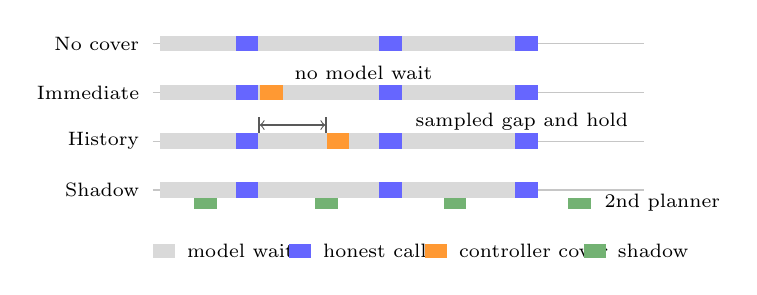
\begin{tikzpicture}[x=.48cm,y=.62cm,font=\scriptsize]
\def\bar#1#2#3#4{\fill[#4] (#1,#3-.16) rectangle (#2,#3+.16);}
\foreach \y/\n in {4/No cover,3/Immediate,2/History,1/Shadow}{
 \node[anchor=east] at (-.1,\y) {\n};
 \draw[gray!45] (0,\y)--(13,\y);
 \bar{0.2}{2.2}{\y}{gray!30}\bar{2.2}{2.8}{\y}{blue!60}
 \bar{2.8}{6.0}{\y}{gray!30}\bar{6.0}{6.6}{\y}{blue!60}
 \bar{6.6}{9.6}{\y}{gray!30}\bar{9.6}{10.2}{\y}{blue!60}}
% immediate cover: right after the honest response
\bar{2.85}{3.45}{3}{orange!80}
\node[anchor=west] at (3.5,3.4) {no model wait};
% history cover: after a sampled gap
\bar{4.6}{5.2}{2}{orange!80}
\draw[|<->|,gray!70!black] (2.8,2.33)--(4.6,2.33);
\node[anchor=west] at (6.7,2.4) {sampled gap and hold};
% shadow chain: its own model waits
\foreach \a in {1.1,4.3,7.7,11.0}{\fill[green!45!black!55] (\a,.62) rectangle (\a+.6,.84);}
\node[anchor=west] at (11.7,.73) {2nd planner};
% legend
\begin{scope}[yshift=-.25cm]
\fill[gray!30] (0,0) rectangle (.6,.3); \node[anchor=west] at (.65,.15) {model wait};
\fill[blue!60] (3.6,0) rectangle (4.2,.3); \node[anchor=west] at (4.25,.15) {honest call};
\fill[orange!80] (7.2,0) rectangle (7.8,.3); \node[anchor=west] at (7.85,.15) {controller cover};
\fill[green!45!black!55] (11.4,0) rectangle (12.0,.3); \node[anchor=west] at (12.05,.15) {shadow};
\end{scope}
\end{tikzpicture}
\caption{Dispatchers in the live study. Honest calls follow a model wait. Immediate cover follows the previous response without one, which label-free gap removal exploits. History-matched cover samples a training gap and response hold. Shadow calls come from a second planner, so their gaps are model waits too.}\label{fig:dispatch}
\end{figure}
